% Provenance (never printed): see sources/outline_sources.md (Year 3: the main
% field and its secular variation, rock magnetism, palaeomagnetic poles, apparent
% polar wander, magnetostratigraphy, the geodynamo). Brief: sources/book5/BRIEFS.md,
% ch. 4. Curves and maps from figdata/bachelor-3/igrf_field.py (IGRF-14),
% palaeomag_stats.py (the invented Kesta terrane, its Fisher statistics, the
% Zijderveld specimen and the reference APW path), magnetostratigraphy.py.
% Exercise and problem values in the Book 5 scratch calculator calc/ch04.py.
\chapter{Geomagnetismo e paleomagnetismo}\label{ch:b3:palaeomagnetism}

Um derrame de basalto, em erupção há sessenta milhões de anos, resfriou-se com seus minúsculos grãos de
magnetita fixados paralelamente ao campo da época. Perfurado hoje, orientado no
local, cortado em pequenos cilindros e aquecido
passo a passo numa sala blindada contra o campo atual, ainda revela quão longe
ele então se encontrava do polo e para que lado se voltava. Milhares de tais
medições, de todos os continentes e de todas as idades, mostraram como os continentes
se deslocaram antes que nascessem os assoalhos oceânicos que registram seu movimento, e em
que ordem o campo se inverteu através das camadas de uma seção sedimentar.
Este capítulo descreve o campo como é hoje, como as rochas o registram,
como uma direção é extraída e tem sua média calculada, e o que um polo paleomagnético diz
sobre o movimento de uma placa.

\begin{recall}
A Terra como um ímã e a declinação magnética estão nos livros de física,
nos volumes escolares; domínios magnéticos, histerese, remanência e a
temperatura de Curie no volume do terceiro ano; o campo de um dipolo magnético no
volume do primeiro ano. Inversões magnéticas e as polaridades normal e reversa foram
vistas no 11º ano. O grande círculo e o triângulo esférico foram definidos no
volume do primeiro ano, no seu capítulo sobre astronomia esférica; o cron de polaridade,
a escala de tempo de polaridade geomagnética, a anomalia magnética marinha e as rotações finitas
em torno de um polo de Euler no seu capítulo sobre cinemática de placas na esfera;
a trajetória de ponto quente no seu capítulo sobre pontos quentes. Os harmônicos esféricos e as
funções de Legendre normalizadas de Schmidt $P_n^m$ foram usadas para a gravidade no
capítulo sobre gravidade e a forma da Terra (o \cref{ch:b3:gravity-geodesy}).
\end{recall}

\section{O campo principal}

\begin{definition}[Campo geomagnético principal; dipolo axial geocêntrico]\label{def:b3:palaeomagnetism:main-field}
O \emph{campo geomagnético principal}\index{campo geomagnético principal} é a parte do
campo magnético terrestre gerado no interior da Terra, no seu núcleo externo
líquido de ferro; muda de anos a milhões de anos, ao contrário dos campos da
ionosfera e da magnetosfera, que mudam de segundos a dias. O
\emph{dipolo axial geocêntrico}\index{dipolo axial geocêntrico} é o campo de um
dipolo magnético colocado no centro da Terra e alinhado com o seu eixo
de rotação, apontando para o sul, de modo que suas linhas de campo saem do hemisfério sul e
entram no hemisfério norte.
\end{definition}

Em qualquer ponto da superfície, o campo $\mathbf F$ é um vetor. Ele é descrito
em um referencial local (figura abaixo): $X$ para o norte geográfico, $Y$ para o
leste, $Z$ para baixo. Sua componente horizontal é $H = \sqrt{X^2 + Y^2}$, sua
intensidade total $F = |\mathbf F|$, sua declinação magnética $D$, o ângulo do
norte geográfico até $\mathbf H$, contado no sentido horário, e sua inclinação $I$, o
ângulo da horizontal até $\mathbf F$.

\begin{definition}[Inclinação magnética]\label{def:b3:palaeomagnetism:inclination}
A \emph{inclinação magnética}\index{inclinação magnética} $I$ do campo em
um ponto é o ângulo entre o vetor do campo e o plano horizontal,
positivo quando o campo aponta para baixo: $\tan I = Z/H$, com $-\ang{90} \le I
\le \ang{90}$.
\end{definition}

\begin{omfigure}
\begin{tikzpicture}[font=\small, x=1cm, y=1cm, >={Stealth[length=5pt]}]
% schematic; X = 3.0, Y = 1.0 (along the oblique east axis), Z = 2.4
\coordinate (O) at (0,0);
\coordinate (E) at (0.9,0.65);
\fill[gray!12] (-0.6,-0.43) -- (3.6,-0.43) -- ($(3.6,-0.43)+2.2*(E)$) -- ($(-0.6,-0.43)+2.2*(E)$) -- cycle;
\draw[->] (O) -- (4.0,0) node[right] {$X$, norte geográfico};
\draw[->] (O) -- ($1.9*(E)$) node[above right] {$Y$, leste};
\draw[->] (O) -- (0,-3.0) node[below] {$Z$, para baixo};
\coordinate (Hh) at ($(3.0,0)+1.0*(E)$);
\coordinate (F) at ($(Hh)+(0,-2.4)$);
\draw[densely dashed, gray] (3.0,0) -- (Hh);
\draw[densely dashed, gray] ($1.0*(E)$) -- (Hh);
\draw[densely dashed, gray] (Hh) -- (F);
\draw[densely dashed, gray] (0,-2.4) -- (F);
\draw[very thick, ->, blue!60!black] (O) -- (Hh) node[pos=0.3, above, sloped] {$\mathbf H$};
\draw[very thick, ->, red!70!black] (O) -- (F) node[pos=0.55, below left] {$\mathbf F$};
\draw[thick] (1.25,0) arc[start angle=0, end angle=9.46, radius=1.25];
\node at (1.62,0.13) {$D$};
\draw[thick, red!70!black] ($0.36*(Hh)$) to[bend left=30] ($0.3*(F)$);
\node[red!70!black] at (1.62,-0.42) {$I$};
\end{tikzpicture}

\par\smallskip{\small Os elementos do campo em um ponto: componentes norte $X$, leste
$Y$ e para baixo $Z$, a componente horizontal $\mathbf H$, o campo total
$\mathbf F$, a declinação magnética $D$ (no plano horizontal, em cinza)
e a inclinação $I$ (no plano vertical que contém $\mathbf
F$).}\label{fig:b3:palaeomagnetism:elements}
\end{omfigure}

\begin{theorem}[Fórmula do dipolo]\label{thm:b3:palaeomagnetism:dipole}
Na superfície de uma esfera de raio $a$, o campo de um \omterm{def:b3:palaeomagnetism:main-field}{dipolo axial
geocêntrico} de momento $m$ tem, na latitude $\lambda$,
\[
  H = B_0\cos\lambda,\qquad Z = 2B_0\sin\lambda,\qquad
  F = B_0\sqrt{1 + 3\sin^2\lambda},\qquad
  \tan I = 2\tan\lambda,\qquad D = 0,
\]
onde $B_0 = \mu_0 m/(4\pi a^3)$ é o campo no equador. Esta é a
\emph{fórmula do dipolo}\index{fórmula do dipolo}.
\end{theorem}

\begin{proof}
Fora de suas fontes, o campo deriva de um potencial escalar magnético,
$\mathbf B = -\nabla V$. Para um dipolo de momento $m$ apontando ao longo de $-z$, o
sul geográfico, $V = -\mu_0 m\cos\theta/(4\pi r^2)$, com $\theta$ a
colatitude. Em coordenadas esféricas, $B_r = -\partial V/\partial r =
-2\mu_0 m\cos\theta/(4\pi r^3)$ e $B_\theta = -(1/r)\,\partial V/\partial\theta =
-\mu_0 m\sin\theta/(4\pi r^3)$, e $B_\varphi = 0$. Em $r = a$, a componente para baixo
é $Z = -B_r = 2B_0\cos\theta = 2B_0\sin\lambda$, e como
$\mathbf e_\theta$ aponta para o sul, a componente para o norte é $X = -B_\theta =
B_0\sin\theta = B_0\cos\lambda$, com $Y = 0$. Então $H = X$, $D = 0$, $\tan I =
Z/H = 2\tan\lambda$ e $F^2 = B_0^2(\cos^2\lambda + 4\sin^2\lambda) =
B_0^2(1 + 3\sin^2\lambda)$.
\end{proof}

A inclinação é zero no equador, \ang{90} no polo norte e
negativa no hemisfério sul; a intensidade nos polos é o dobro da existente no
equador. O campo real não é um dipolo perfeito e é descrito, como a gravidade,
por harmônicos esféricos.

\begin{definition}[Campo Geomagnético Internacional de Referência]\label{def:b3:palaeomagnetism:igrf}
O \emph{Campo Geomagnético Internacional de Referência}\index{Campo Geomagnético Internacional de Referência}
(IGRF) é o modelo acordado internacionalmente do
campo principal: o potencial, na superfície e acima dela,
\[
  V(r,\theta,\varphi) = a\sum_{n=1}^{N}\Bigl(\frac ar\Bigr)^{n+1}\sum_{m=0}^{n}
  \bigl(g_n^m\cos m\varphi + h_n^m\sin m\varphi\bigr)P_n^m(\cos\theta),
\]
com $a = \qty{6371.2}{km}$, $\mathbf B = -\nabla V$, e coeficientes de Gauss
$g_n^m$, $h_n^m$ (em \unit{nT}) fornecidos a cada cinco anos desde 1900, junto
com sua taxa de variação nos cinco anos seguintes.
\end{definition}
% ledger: geomag5:igrf, data:b5-igrf

O modelo é mantido pela International Association of Geomagnetism and
Aeronomy; sua décima quarta geração foi concluída em novembro de 2024 e é
truncada no grau $N = 13$. O primeiro termo, $g_1^0$, é o dipolo axial:
comparando com a prova acima, $B_0 = -g_1^0$, e $g_1^0 = \qty{-29350}{nT}$
em 2025. Com os outros dois termos de grau 1, o dipolo é inclinado; seu eixo encontra
a superfície no polo geomagnético norte, em \ang{80.79}\,N, \ang{72.76}\,O em
2025, e seu momento é $m = 4\pi a^3\sqrt{(g_1^0)^2 + (g_1^1)^2 +
(h_1^1)^2}/\mu_0 = \qty{7.69e22}{A.m^2}$.
% ledger: data:b5-igrf

\begin{omfigure}
\begin{tikzpicture}
\begin{groupplot}[group style={group size=1 by 2, vertical sep=1.4cm},
  ommap, width=0.96\linewidth, xtick={-180,-120,...,180}, ytick={-60,0,60},
  unbounded coords=jump, title style={font=\small, yshift=-1ex}]
\nextgroupplot[title={(a) inclinação, a cada \ang{20}}]
% computed in figdata/bachelor-3/igrf_field.py; ledger: data:b5-igrf, data:ne-land
\addplot[fill=omLithAlluv, draw=black!45, line width=0.2pt, forget plot] table {figdata/out/shared-geo-land.dat};
\addplot[red!70!black, line width=0.5pt] table[x=x, y=y] {figdata/out/bachelor-3-igrf_field-incl.dat};
\addplot[black, line width=1.1pt] table[x=x, y=y] {figdata/out/bachelor-3-igrf_field-dipeq.dat};
\addplot[draw=none, nodes near coords, point meta=explicit,
  every node near coord/.style={font=\tiny, fill=white, inner sep=0.6pt, anchor=center}]
  table[x=x, y=y, meta=lev] {figdata/out/bachelor-3-igrf_field-inclab.dat};
\nextgroupplot[title={(b) intensidade total, a cada \qty{5000}{nT}}]
\addplot[fill=omLithAlluv, draw=black!45, line width=0.2pt, forget plot] table {figdata/out/shared-geo-land.dat};
\addplot[blue!60!black, line width=0.5pt] table[x=x, y=y] {figdata/out/bachelor-3-igrf_field-intens.dat};
\addplot[draw=none, nodes near coords, point meta=explicit,
  every node near coord/.style={font=\tiny, fill=white, inner sep=0.6pt, anchor=center}]
  table[x=x, y=y, meta=lev] {figdata/out/bachelor-3-igrf_field-intlab.dat};
\addplot[only marks, mark=x, mark size=3pt, line width=1pt, black] table {figdata/out/bachelor-3-igrf_field-fmin.dat};
\end{groupplot}
\end{tikzpicture}

\par\smallskip{\small O campo principal em 2025, segundo o 14.º IGRF, na
superfície da esfera de raio \qty{6371.2}{km}. (a) Inclinação em graus;
a linha espessa, $I = 0$, é o equador de mergulho. (b) Intensidade total em \unit{nT};
a cruz marca o campo mais fraco, cerca de \qty{22100}{nT}, sobre o Atlântico
Sul, contra cerca de \qty{66600}{nT} no mais forte, ao sul da
Austrália.}\label{fig:b3:palaeomagnetism:igrf-maps}
\end{omfigure}

Os mapas acima mostram o quanto o campo se afasta de um dipolo. O equador de mergulho
oscila até cerca de \ang{12} do equador geográfico, e a intensidade,
que um dipolo tornaria uniforme ao longo de um paralelo, varia por um fator de
três, com uma ampla depressão sobre o Atlântico Sul.
% ledger: data:b5-igrf

\begin{definition}[Variação secular]\label{def:b3:palaeomagnetism:secular}
A \emph{variação secular}\index{variação secular} é a lenta mudança do
campo principal com o tempo, em escalas de anos a séculos, medida pela taxa de
variação de seus coeficientes de Gauss ou de seus elementos em um lugar.
\end{definition}

Nos últimos 125 anos o momento de dipolo caiu de
\qty{8.32e22}{A.m^2} para \qty{7.69e22}{A.m^2}, uma redução de \qty{7.6}{\percent}, e o
polo geomagnético norte deslocou-se de \ang{78.61}\,N, \ang{68.79}\,O até sua
posição atual (figura abaixo); $g_1^0$ ainda cresce \qty{12.6}{nT} por ano,
um enfraquecimento do dipolo.
% ledger: data:b5-igrf

\begin{omfigure}
\begin{tikzpicture}
\begin{groupplot}[group style={group size=2 by 1, horizontal sep=1.7cm},
  omrecord, width=0.47\linewidth, height=0.4\linewidth, xmin=1895, xmax=2030,
  xtick={1900,1950,2000}, xticklabel style={/pgf/number format/1000 sep=},
  xlabel={ano}]
\nextgroupplot[ylabel={momento de dipolo (\qty{e22}{A.m^2})}, ymin=7.6, ymax=8.4]
% computed in figdata/bachelor-3/igrf_field.py; ledger: data:b5-igrf
\addplot[omDef, thick, mark=*, mark size=1pt] table[x=year, y=M] {figdata/out/bachelor-3-igrf_field-dipole.dat};
\nextgroupplot[ylabel={latitude do polo (\unit{\degree}\,N)}, ymin=78, ymax=81.5]
\addplot[red!70!black, thick, mark=*, mark size=1pt] table[x=year, y=plat] {figdata/out/bachelor-3-igrf_field-dipole.dat};
\end{groupplot}
\end{tikzpicture}

\par\smallskip{\small A parte de dipolo do campo principal, 1900--2025, a cada cinco
anos, segundo o IGRF: seu momento (à esquerda) e a latitude do polo
geomagnético norte (à direita).}\label{fig:b3:palaeomagnetism:dipole}
\end{omfigure}

De onde vem o campo? Um ímã permanente está descartado: a temperatura
de Curie da magnetita é de cerca de \qty{580}{\celsius} e a da hematita
\qty{675}{\celsius}, e o interior da Terra é muito mais quente. O campo é
regenerado continuamente pelo movimento do líquido condutor do núcleo
externo.
% ledger: tarduno:curie

\begin{definition}[Geodínamo]\label{def:b3:palaeomagnetism:geodynamo}
O \emph{geodínamo}\index{geodínamo} é o processo autossustentado pelo qual a
convecção da liga de ferro líquida, eletricamente condutora, do núcleo externo,
desviada pela rotação da Terra, induz correntes elétricas cujo campo
magnético se mantém contra o decaimento ôhmico.
\end{definition}

\begin{proposition}[Equação de indução]\label{prop:b3:palaeomagnetism:induction}
Em um condutor de difusividade magnética $\eta = 1/(\mu_0\sigma)$ que se move com a
velocidade $\mathbf u$, o campo magnético obedece a
\[
  \frac{\partial\mathbf B}{\partial t} = \nabla\times(\mathbf u\times\mathbf B)
  + \eta\nabla^2\mathbf B .
\]
\end{proposition}
\admitted

O primeiro termo estica e torce as linhas de campo transportadas pelo escoamento; o
segundo faz o campo decair, em um corpo de tamanho $L$, em um tempo da ordem de
$L^2/\eta$. Um dínamo funciona quando o escoamento regenera o campo mais depressa do que
o campo se difunde para longe. Simulações computacionais de uma casca de fluido em convecção e rotação
reproduzem um dipolo axial dominante e, de tempos em tempos, uma inversão; mas as
equações do \omterm{def:b3:palaeomagnetism:geodynamo}{geodínamo}, acopladas às do escoamento, estão além deste
livro. Além das inversões completas, o registro guarda eventos mais curtos.

\begin{definition}[Excursão geomagnética]\label{def:b3:palaeomagnetism:excursion}
Uma \emph{excursão geomagnética}\index{excursão geomagnética} é um grande
desvio da direção do campo em relação à do dipolo axial, sendo o
\omterm{def:b3:palaeomagnetism:vgp}{polo geomagnético virtual} (ver a \cref{def:b3:palaeomagnetism:vgp}) afastando-se muito
do polo geográfico, que retorna à polaridade original em vez de
completar uma inversão.
\end{definition}

\section{Como as rochas registram o campo}

Minerais ferromagnéticos em sentido amplo, sobretudo magnetita em rochas ígneas
e hematita em sedimentos vermelhos, carregam uma remanência. Acima de sua temperatura de Curie
um grão não possui nenhuma; abaixo dela, um grão pequeno é um único domínio magnético cujo
momento se inverte entre suas direções fáceis, por ativação térmica, após um
tempo de relaxação
\[
  \tau = \frac1C\exp\Bigl(\frac{K V}{k_B T}\Bigr),
\]
em que $K$ é a energia de anisotropia por unidade de volume, $V$ o volume do grão
e $C$ um fator de frequência. Esta é a lei de relaxação de Néel, admitida aqui. Como
$\tau$ cresce exponencialmente à medida que $T$ diminui, um grão passa por um estreito intervalo
de temperatura, da condição de inverter o momento livremente para a de mantê-lo por bilhões de
anos.

\begin{definition}[Temperatura de bloqueio]\label{def:b3:palaeomagnetism:blocking}
A \emph{temperatura de bloqueio}\index{temperatura de bloqueio} de um grão magnético
é a temperatura abaixo da qual seu tempo de relaxação excede o tempo do
experimento, de modo que seu momento permanece fixo: ao resfriar através dela, o grão
registra o campo; ao aquecer através dela em campo nulo, o grão perde esse
registro.
\end{definition}

\begin{definition}[Magnetização remanente natural, térmica, detrítica e química]\label{def:b3:palaeomagnetism:nrm}
A \emph{magnetização remanente natural}\index{magnetização remanente natural}
(NRM) de uma rocha é a remanência que ela carrega à medida que é coletada, a soma de
componentes adquiridas em tempos diferentes. Uma \emph{magnetização
termorremanente}\index{magnetização termorremanente} (TRM) é adquirida durante o resfriamento
através das \omterm{def:b3:palaeomagnetism:blocking}{temperaturas de bloqueio} em um campo, como em um derrame de lava ou
uma intrusão. Uma \emph{magnetização remanente detrítica}\index{magnetização remanente detrítica}
(DRM) é adquirida quando grãos magnéticos que se depositam na água, ou no
sedimento úmido logo abaixo de sua superfície, giram para se alinhar ao campo antes de
ficarem fixados. Uma \emph{magnetização remanente química}\index{magnetização remanente química}
(CRM) é adquirida quando um mineral magnético cresce, através de um
volume de bloqueio, em um campo, como faz a hematita quando se forma uma camada vermelha.
\end{definition}

Uma TRM registra o campo no momento do resfriamento; uma DRM, dentro do tempo que o
sedimento leva para se compactar; uma CRM, sempre que o mineral cresceu, o que pode ter sido bem
depois da deposição. Um reaquecimento posterior, ou o campo atual atuando por muito tempo
sobre grãos de tempo de relaxação curto, acrescenta uma componente secundária por cima: uma
remanência viscosa ao longo do campo recente.

\section{Do espécime à direção}

Testemunhos orientados são perfurados em vários sítios de uma formação, alguns testemunhos por
sítio, e cortados em espécimes de alguns centímetros cúbicos. A NRM de cada espécime é
medida e, em seguida, progressivamente removida.

\begin{definition}[Desmagnetização por etapas]\label{def:b3:palaeomagnetism:demag}
A \emph{desmagnetização por etapas}\index{desmagnetização por etapas} é a remoção
da remanência de um espécime em etapas de intensidade crescente, medindo o
vetor remanescente após cada uma: por aquecimento a temperaturas crescentes e resfriamento
em campo nulo (desmagnetização térmica), que remove antes as componentes de
\omterm{def:b3:palaeomagnetism:blocking}{temperatura de bloqueio} mais baixa, ou por campos magnéticos alternados de valor de pico
crescente que decaem até zero (desmagnetização por campo alternado), que remove
antes as de menor coercividade.
\end{definition}

\begin{definition}[Diagrama de Zijderveld; magnetização remanente característica]\label{def:b3:palaeomagnetism:zijderveld}
Um \emph{diagrama de Zijderveld}\index{diagrama de Zijderveld} representa os pontos finais do
vetor de remanência restante após cada etapa de desmagnetização em dois planos
ao mesmo tempo, o horizontal (norte contra leste) e um vertical (norte
contra para baixo), com um eixo norte comum. Uma componente removida isoladamente ao longo de um intervalo
de etapas aparece como um segmento de reta; um segmento que termina na origem é a
\emph{magnetização remanente característica}\index{magnetização remanente característica}
(ChRM), a componente mais estável, interpretada como a primária
quando os testes permitem.
\end{definition}

O espécime da figura abaixo carrega duas componentes: uma sobreimpressão viscosa
ao longo do campo atual, removida até \qty{300}{\celsius}, e uma ChRM
desbloqueada de 300 a \qty{580}{\celsius}, a temperatura de Curie da magnetita.
Acima de \qty{300}{\celsius}, ambas as projeções seguem em linha reta até a origem; a
direção desse segmento é a da ChRM.

\begin{omfigure}
\begin{tikzpicture}
\begin{groupplot}[group style={group size=2 by 1, horizontal sep=1.3cm},
  width=0.5\linewidth]
\nextgroupplot[axis lines=middle, axis equal image, xmin=-4, xmax=36, ymin=-4, ymax=42,
  y dir=reverse, xlabel={N}, ylabel={L, baixo}, tick label style={font=\scriptsize},
  xtick={0,10,20,30}, ytick={10,20,30,40}, label style={font=\small},
  xlabel style={at={(ticklabel* cs:1.0)}, anchor=west},
  ylabel style={at={(ticklabel* cs:1.0)}, anchor=north west},
  title={(a) Diagrama de Zijderveld (\unit{mA/m})}, title style={font=\small, yshift=1ex},
  clip=false, legend style={font=\scriptsize, at={(0.13,0.03)}, anchor=south west, cells={anchor=west}}]
% computed in figdata/bachelor-3/palaeomag_stats.py (synthetic specimen)
\addplot[black, mark=*, mark size=1.5pt] table[x=N, y=E] {figdata/out/bachelor-3-palaeomag_stats-zij.dat};
\addlegendentry{horizontal: N, L}
\addplot[black, mark=o, mark size=1.7pt, fill=white] table[x=N, y=Down] {figdata/out/bachelor-3-palaeomag_stats-zij.dat};
\addlegendentry{vertical: N, baixo}
\node[font=\scriptsize, anchor=south west] at (axis cs:32.2,18.1) {\qty{20}{\celsius}};
\node[font=\scriptsize, anchor=north west] at (axis cs:32.2,38.2) {\qty{20}{\celsius}};
\node[font=\scriptsize, anchor=south] at (axis cs:25.8,17.6) {300};
\node[font=\scriptsize, anchor=east] at (axis cs:25.0,24.6) {300};
\node[font=\scriptsize, anchor=south east] at (axis cs:-0.5,-0.5) {580};
\nextgroupplot[axis equal image, hide axis, clip=false, xmin=-1.12, xmax=1.12, ymin=-1.12, ymax=1.18,
  title={(b) sítio A, projeção de áreas iguais, hemisfério inferior}, title style={font=\small, yshift=1ex}]
\addplot[black, domain=0:360, samples=145, thin] ({cos(x)},{sin(x)});
\draw[black] (axis cs:0,1) -- (axis cs:0,1.08) node[above, font=\scriptsize] {N};
\draw[black] (axis cs:1,0) -- (axis cs:1.06,0);
\draw[black] (axis cs:0,-1) -- (axis cs:0,-1.06);
\draw[black] (axis cs:-1,0) -- (axis cs:-1.06,0);
\draw[black] (axis cs:-0.04,0) -- (axis cs:0.04,0) (axis cs:0,-0.04) -- (axis cs:0,0.04);
\addplot[only marks, mark=*, mark size=1.6pt, black] table[x=x, y=y] {figdata/out/bachelor-3-palaeomag_stats-dirsA.dat};
\addplot[omDef, thick] table[x=x, y=y] {figdata/out/bachelor-3-palaeomag_stats-cone.dat};
\addplot[only marks, mark=star, mark size=3.5pt, omDef, line width=0.9pt] table[x=x, y=y] {figdata/out/bachelor-3-palaeomag_stats-meanA.dat};
\end{groupplot}
\end{tikzpicture}

\par\smallskip{\small (a) Desmagnetização térmica de um espécime sintético, de
\qty{20}{\celsius} a \qty{580}{\celsius}: pontos cheios, a projeção
horizontal; pontos vazios, a vertical. (b) As seis direções de ChRM do sítio A
do problema de fim de semana (pontos), sua média (estrela) e seu cone de
confiança de 95 por cento (círculo).}\label{fig:b3:palaeomagnetism:zijderveld}
\end{omfigure}

As direções dos espécimes de um sítio se dispersam em torno de uma média, e a
estatística dessa dispersão é a de uma distribuição sobre a esfera.

\begin{proposition}[Distribuição de Fisher]\label{prop:b3:palaeomagnetism:fisher}
A \emph{distribuição de Fisher}\index{distribuição de Fisher} de precisão
de parâmetro $\kappa > 0$ em torno de uma direção média atribui a um vetor unitário a
densidade de probabilidade, por unidade de ângulo sólido,
\[
  f(\theta) = \frac{\kappa}{4\pi\sinh\kappa}\,e^{\kappa\cos\theta},
\]
em que $\theta$ é o seu ângulo em relação à média. Dados $N$ vetores unitários $\mathbf u_i$
extraídos dela, com resultante $\mathbf R = \sum\mathbf u_i$ de comprimento $R$, a
melhor estimativa da direção média é a de $\mathbf R$; a precisão é
estimada por $k = (N - 1)/(N - R)$; e a verdadeira média encontra-se, com probabilidade
$1 - p$, dentro do ângulo $\alpha_{1-p}$ da média estimada, em que
\[
  \cos\alpha_{1-p} = 1 - \frac{N - R}{R}\Bigl[\Bigl(\frac1p\Bigr)^{1/(N-1)} - 1\Bigr].
\]
\end{proposition}
\admitted

\begin{definition}[Alfa-95]\label{def:b3:palaeomagnetism:a95}
O \emph{alfa-95}\index{alfa-95} ($\alpha_{95}$) de uma direção média é o
semiângulo de seu cone de confiança de 95 por cento, o ângulo $\alpha_{1-p}$ da
\cref{prop:b3:palaeomagnetism:fisher} para $p = 0.05$.
\end{definition}

A densidade integra-se a um: com $\mathrm d\Omega = 2\pi\sin\theta\,\mathrm
d\theta$, $\int_0^\pi f\,2\pi\sin\theta\,\mathrm d\theta =
\frac{\kappa}{2\sinh\kappa}\cdot\frac{e^\kappa - e^{-\kappa}}{\kappa} = 1$. Calcula-se a média das direções como vetores unitários
nunca como ângulos: a média das declinações \ang{350} e \ang{10} é
norte, não sul. Um $k$ grande significa um agrupamento compacto, e $\alpha_{95}$ diminui
aproximadamente como $1/\sqrt{kN}$.

\begin{method}[Testes de campo de uma direção paleomagnética]\label{met:b3:palaeomagnetism:tests}
Pode-se mostrar que uma ChRM é anterior a um evento por meio de um teste feito em campo.
\begin{itemize}
  \item \textbf{Teste da dobra.} Sítios em ambos os flancos de uma dobra: se as direções
        se agrupam melhor depois que os estratos são rotacionados de volta à horizontal do que
        antes, a magnetização é anterior ao dobramento.
  \item \textbf{Teste de reversão.} Se uma formação registra as duas polaridades, a média
        das direções reversas, invertida, deve coincidir com a média das
        normais dentro de seus cones de confiança; uma sobreimpressão viscosa não
        removida enviesaria as duas no mesmo sentido e quebraria a antipodalidade.
  \item \textbf{Teste do contato cozido.} Um dique aquece a rocha encaixante ao
        seu lado, que adquire uma nova TRM: se a rocha cozida carrega a direção do dique
        e a rocha encaixante mais distante, uma direção diferente, a magnetização do dique
        não foi reajustada desde que ele resfriou.
\end{itemize}
\end{method}

\section{Polos e placas}

Se o campo, médio sobre alguns milhares de anos para suavizar a \omterm{def:b3:palaeomagnetism:secular}{variação
secular}, é um \omterm{def:b3:palaeomagnetism:main-field}{dipolo axial geocêntrico}, então a \omterm{thm:b3:palaeomagnetism:dipole}{fórmula do dipolo} transforma uma
inclinação média em uma latitude, e a declinação média aponta para o polo.

\begin{definition}[Paleolatitude; polo geomagnético virtual]\label{def:b3:palaeomagnetism:vgp}
A \emph{paleolatitude}\index{paleolatitude} de um sítio é a latitude
$\lambda$ dada por sua inclinação média pela \omterm{thm:b3:palaeomagnetism:dipole}{fórmula do dipolo}, $\tan I =
2\tan\lambda$. O \emph{polo geomagnético virtual}\index{polo geomagnético virtual}
(VGP) de uma direção $(D, I)$ observada em um sítio é o polo norte do
dipolo geocêntrico que produziria essa direção ali.
\end{definition}

\begin{theorem}[O polo de uma direção]\label{thm:b3:palaeomagnetism:pole}
Seja um sítio de latitude $\lambda_s$ e longitude $\varphi_s$ e uma
direção média $(D, I)$. Seja $p$ a paleocolatitude, $\cot p = \tfrac12\tan I$,
com $0 \le p \le \ang{180}$. O \omterm{def:b3:palaeomagnetism:vgp}{polo geomagnético virtual} tem latitude
$\lambda_p$ e longitude $\varphi_p$ dadas por
\[
  \sin\lambda_p = \sin\lambda_s\cos p + \cos\lambda_s\sin p\cos D,\qquad
  \sin\beta = \frac{\sin p\sin D}{\cos\lambda_p},
\]
com $\varphi_p = \varphi_s + \beta$ se $\cos p \ge \sin\lambda_s\sin\lambda_p$,
e $\varphi_p = \varphi_s + \ang{180} - \beta$ caso contrário.
\end{theorem}

\begin{proof}
Na esfera, o sítio $S$, o polo norte geográfico $N$ e o VGP $P$ formam um
triângulo esférico (figura abaixo). O lado $NS$ é a colatitude do sítio,
$\ang{90} - \lambda_s$; o lado $SP$ é a distância angular do sítio ao
polo do dipolo, que a \omterm{thm:b3:palaeomagnetism:dipole}{fórmula do dipolo} dá como $p$, pois a latitude magnética do sítio
é $\ang{90} - p$; e o ângulo em $S$, entre
as direções para $N$ e $P$, é a declinação $D$. A lei dos cossenos para o
lado $NP = \ang{90} - \lambda_p$ dá a primeira relação; a lei dos senos,
$\sin\beta/\sin p = \sin D/\sin(\ang{90} - \lambda_p)$, dá o ângulo $\beta$
em $N$, a diferença de longitudes. O seno determina $\beta$ apenas a menos de
seu suplemento: a lei dos cossenos para o lado $SP$, $\cos p = \sin\lambda_s
\sin\lambda_p + \cos\lambda_s\cos\lambda_p\cos\beta$, mostra que $\cos\beta \ge
0$ exatamente quando $\cos p \ge \sin\lambda_s\sin\lambda_p$.
\end{proof}

\begin{omfigure}
\begin{tikzpicture}[font=\small, >={Stealth[length=5pt]}]
\draw[gray!60] (0,0) circle (2.6);
\draw[gray!50, densely dashed] (-2.6,0) arc[start angle=180, end angle=360, x radius=2.6, y radius=0.7];
\coordinate (N) at (0,2.6);
\coordinate (S) at (-1.2,0.25);
\coordinate (P) at (1.25,1.65);
\fill (N) circle (1.6pt) node[above] {$N$};
\fill (S) circle (1.6pt) node[below left] {$S$ (sítio)};
\fill[omDef] (P) circle (1.8pt) node[right] {$P$ (VGP)};
\draw[thick] (N) to[bend right=12] node[left, pos=0.55] {$\ang{90}-\lambda_s$} (S);
\draw[thick, omDef] (S) to[bend left=10] node[below right, pos=0.55] {$p$} (P);
\draw[thick, blue!60!black] (N) to[bend left=12] node[above right, pos=0.45] {$\ang{90}-\lambda_p$} (P);
\draw ($(S)!0.2!(N)$) to[bend left=35] ($(S)!0.2!(P)$);
\node[inner sep=1pt] at (-0.61,0.86) {$D$};
\draw ($(N)!0.18!(S)$) to[bend right=40] node[below, pos=0.5, inner sep=2pt] {$\beta$} ($(N)!0.18!(P)$);
\end{tikzpicture}

\par\smallskip{\small O triângulo esférico do \omterm{def:b3:palaeomagnetism:vgp}{polo geomagnético virtual}:
polo geográfico norte $N$, sítio $S$, polo $P$. O ângulo no sítio é a
declinação $D$; o ângulo no polo $N$ é a diferença de longitudes
$\beta$.}\label{fig:b3:palaeomagnetism:vgp}
\end{omfigure}

O cone $\alpha_{95}$ em torno da direção média transforma-se num oval em torno do polo,
de semieixos $\mathrm dp = \tfrac12\alpha_{95}(1 + 3\cos^2p)$ ao longo do grande
círculo a partir do sítio, e $\mathrm dm = \alpha_{95}\sin p/\cos I$ perpendicularmente a ele. Um
polo médio de vários sítios de uma formação, cada um um VGP, é um polo paleomagnético com
cone próprio, $A_{95}$. Rochas de mesma idade numa mesma placa rígida dão o
mesmo polo; rochas de idades diferentes, polos diferentes.

\begin{definition}[Deriva polar aparente; trajetória de deriva polar aparente]\label{def:b3:palaeomagnetism:apw}
A \emph{deriva polar aparente}\index{deriva polar aparente} é a variação, com a idade das rochas,
do polo paleomagnético de uma placa vista a partir dessa mesma placa, tomada como fixa.
Uma \emph{trajetória de deriva polar aparente}\index{trajetória de deriva polar aparente}
é a curva que une os polos paleomagnéticos de uma placa em ordem
de idade.
\end{definition}

O polo não se desloca: é a placa que se move, e a trajetória registra esse movimento em
sentido inverso. Duas placas que se afastaram têm trajetórias diferentes para o tempo
anterior à separação, e cada trajetória é girada sobre a outra pela rotação finita
que fecha o oceano entre elas. Um polo paleomagnético fixa a
latitude de um bloco e sua orientação, mas não sua longitude: uma rotação do
bloco em torno do eixo de rotação não altera nenhuma das duas.

Um bloco deslocado, um terreno, é testado contra a trajetória da placa estável de
que faz parte agora. A partir do polo de referência da idade correta calcula-se a
direção esperada $(D_x, I_x)$ no sítio, por meio do \cref{thm:b3:palaeomagnetism:pole}
lido ao contrário. Uma rotação horária do bloco em torno de um eixo vertical é
medida por $R = D_o - D_x$, seu deslocamento em direção ao polo por $P = \lambda_x -
\lambda_o$, a diferença entre as \omterm{def:b3:palaeomagnetism:vgp}{paleolatitudes} esperada e observada; o
erro de uma declinação é de cerca de $\Delta D = \arcsin(\sin\alpha_{95}/\cos I)$,
e os erros se combinam como a raiz da soma de seus quadrados. A cadeia Havaí--Imperador
foi submetida a esse teste no volume do primeiro ano, em seu capítulo sobre pontos quentes:
as \omterm{def:b3:palaeomagnetism:vgp}{paleolatitudes} medidas nos montes submarinos de Imperador mostraram o próprio ponto quente
deslocando-se para o sul, em mais de \qty{40}{mm/yr} entre 81 e \qty{47}{Ma}.
% ledger: tarduno:emperor

\begin{omfigure}
\begin{tikzpicture}
\begin{axis}[axis equal image, hide axis, width=0.62\linewidth,
  xmin=-0.62, xmax=0.62, ymin=-0.62, ymax=0.62, unbounded coords=jump,
  legend style={font=\scriptsize, at={(1.03,0.5)}, anchor=west, cells={anchor=west}}]
% computed in figdata/bachelor-3/palaeomag_stats.py (invented continent and terrane)
\addplot[gray!50, line width=0.3pt, forget plot] table[x=x, y=y] {figdata/out/bachelor-3-palaeomag_stats-graticule.dat};
\addplot[black, line width=0.6pt, domain=0:360, samples=145, forget plot]
  ({0.5412*cos(x)},{0.5412*sin(x)});
\addplot[draw=none, nodes near coords, point meta=explicit symbolic, forget plot,
  every node near coord/.style={font=\tiny, anchor=center}]
  table[x=x, y=y, meta=lon] {figdata/out/bachelor-3-palaeomag_stats-lonlabels.dat};
\addplot[blue!60!black, line width=0.4pt, forget plot] table[x=x, y=y,
  restrict expr to domain={\thisrow{id}}{0:9}] {figdata/out/bachelor-3-palaeomag_stats-apwcircles.dat};
\addplot[red!70!black, line width=0.4pt, densely dashed, forget plot] table[x=x, y=y,
  restrict expr to domain={\thisrow{id}}{10:19}] {figdata/out/bachelor-3-palaeomag_stats-apwcircles.dat};
\addplot[blue!60!black, thick, mark=square*, mark size=1.6pt] table[x=x, y=y] {figdata/out/bachelor-3-palaeomag_stats-apwref.dat};
\addlegendentry{trajetória de referência, continente estável}
\addplot[red!70!black, thick, mark=triangle*, mark size=2.2pt] table[x=x, y=y] {figdata/out/bachelor-3-palaeomag_stats-apwkesta.dat};
\addlegendentry{VGPs de Kesta A, B, C}
\node[font=\scriptsize, anchor=west] at (axis cs:0.11,-0.135) {\qty{60}{Ma}};
\node[font=\scriptsize, anchor=west] at (axis cs:0.055,-0.07) {30};
\node[font=\scriptsize, anchor=east] at (axis cs:-0.085,-0.02) {4};
\node[font=\scriptsize, anchor=west] at (axis cs:0.035,0.0) {C, 4};
\node[font=\scriptsize, anchor=west] at (axis cs:-0.09,-0.45) {A, \qty{60}{Ma}};
\node[font=\scriptsize, anchor=west] at (axis cs:-0.04,-0.27) {B, 30};
\fill (axis cs:0,0) circle (1pt);
\end{axis}
\end{tikzpicture}

\par\smallskip{\small Diagrama polar de áreas iguais da região polar norte, até
\ang{45}\,N (círculo externo), paralelos a cada \ang{10} a partir de \ang{50}\,N,
meridianos a cada \ang{30} (rotulados em graus leste). Quadrados: a \omterm{def:b3:palaeomagnetism:apw}{trajetória de deriva polar aparente}
de um continente estável fictício, com os círculos $A_{95}$ de seus polos;
triângulos: os polos geomagnéticos virtuais das três formações do
terreno Kesta fictício do problema de fim de semana, com seus círculos $\alpha_{95}$
(tracejados). O polo geográfico é o ponto no centro.}\label{fig:b3:palaeomagnetism:apw}
\end{omfigure}

Um polo que se desloca em relação ao eixo de rotação pode significar que as placas
se moveram ou que a Terra sólida inteira girou sob o eixo de rotação.

\begin{definition}[Deriva polar verdadeira]\label{def:b3:palaeomagnetism:tpw}
A \emph{deriva polar verdadeira}\index{deriva polar verdadeira} é a rotação de toda a
Terra sólida, manto e crosta juntos, em relação ao seu eixo de rotação, causada
por mudanças na distribuição de massa em seu interior. Ela desloca todos os
polos paleomagnéticos de todas as placas em conjunto, pela mesma rotação, enquanto
o movimento das placas desloca os polos de cada placa de modo diferente.
\end{definition}

Ela só se detecta comparando as trajetórias de todas as placas num referencial
independente do eixo de rotação, como o dos pontos quentes; quão grande ela foi ainda é
debatido, e nenhuma taxa é apresentada aqui.

\section{Magnetoestratigrafia}

\begin{definition}[Magnetoestratigrafia]\label{def:b3:palaeomagnetism:magnetostratigraphy}
A \emph{magnetoestratigrafia}\index{magnetoestratigrafia} é a subdivisão de uma
sequência de rochas em zonas de polaridade, intervalos de polaridade normal ou reversa
uniforme, e a datação da sequência pela correspondência de seu padrão de zonas com
o da escala de tempo de polaridade geomagnética.
\end{definition}

Uma reversão é registrada, dentro da resolução da amostragem, em toda parte no
mesmo instante: um limite de reversão numa seção é uma superfície isócrona.
O padrão de zonas, seu número e suas espessuras relativas, é o que se compara;
uma zona isolada poderia ser qualquer cron de sua polaridade. Uma ou duas
idades independentes, de uma cinza vulcânica ou de um fóssil, ancoram a correspondência, e então
cada limite de reversão data a seção. Na figura abaixo, uma seção de
\qty{64}{m} mostra três zonas normais; ajustada aos subcrons normais do
cron C2An, de 3.596 a \qty{2.581}{Ma}, seus limites dão uma taxa de acumulação de
cerca de \qty{40}{m/Myr} abaixo de \qty{20}{m} e \qty{55}{m/Myr} acima.
% ledger: iodp:gpts2004

\begin{omfigure}
\begin{tikzpicture}[font=\small, x=1cm, y=1cm]
% section heights (m) and GPTS ages (Ma) as printed: magnetostratigraphy.py, part ties
% section: y = h / 10 cm; timescale: y = (3.8 - t) * 16 cm
\def\hs{0.1}\def\ts{4.2}
\draw (0,0) rectangle (1,6.4);
\foreach \lo/\hi in {4.2/14.8, 19.7/24.6, 29.2/54.0}
  \fill[black] (0,\lo*\hs) rectangle (1,\hi*\hs);
\foreach \h in {0,10,...,60} \draw (0,\h*\hs) -- (-0.12,\h*\hs) node[left, font=\scriptsize] {\h};
\node[rotate=90, font=\scriptsize] at (-0.95,3.2) {altura na seção (m)};
\node[above, align=center, font=\scriptsize] at (0.5,6.45) {seção};
\draw (5,{(3.8-3.8)*\ts}) rectangle (6,{(3.8-2.3)*\ts});
\foreach \a/\b in {3.596/3.330, 3.207/3.116, 3.032/2.581}
  \fill[black] (5,{(3.8-\a)*\ts}) rectangle (6,{(3.8-\b)*\ts});
\foreach \t in {2.4,2.6,...,3.81} \draw (6,{(3.8-\t)*\ts}) -- (6.12,{(3.8-\t)*\ts})
  node[right, font=\scriptsize] {\pgfmathprintnumber[fixed, fixed zerofill, precision=1]{\t}};
\node[above, align=center, font=\scriptsize] at (5.8,{(3.8-2.3)*\ts+0.05}) {escala de tempo, idade (Ma)};
\foreach \h/\t in {4.2/3.596, 14.8/3.330, 19.7/3.207, 24.6/3.116, 29.2/3.032, 54.0/2.581}
  \draw[omDef, densely dashed] (1,\h*\hs) -- (5,{(3.8-\t)*\ts});
\node[font=\scriptsize, anchor=west] at (6.9,{(3.8-2.81)*\ts}) {C2An.1n};
\node[font=\scriptsize, anchor=west] at (6.9,{(3.8-3.16)*\ts}) {C2An.2n};
\node[font=\scriptsize, anchor=west] at (6.9,{(3.8-3.46)*\ts}) {C2An.3n};
\end{tikzpicture}

\par\smallskip{\small Uma correlação magnetoestratigráfica: as zonas de polaridade
de uma seção fictícia (preto, normal; branco, reversa) correlacionadas com a
escala de tempo de polaridade entre 3.8 e \qty{2.3}{Ma}. As linhas tracejadas unem
cada limite de reversão à sua idade.}\label{fig:b3:palaeomagnetism:magstrat}
\end{omfigure}

\begin{inthelab}[Um laboratório paleomagnético blindado]
\begin{minipage}[t]{0.55\linewidth}\vspace{0pt}
O laboratório é uma sala dentro de uma blindagem magnética, camadas de metal de alta permeabilidade
que reduzem o campo da Terra a uma pequena fração de seu valor, de modo que as
amostras não adquirem nova remanência enquanto são manuseadas. Um paleomagnetista
carrega as amostras, pequenos cilindros de rocha marcados cada um com uma seta de
orientação, sobre uma bandeja longa que as leva, uma após a outra, até um
magnetômetro criogênico, cujos sensores supercondutores, resfriados por hélio líquido,
medem as três componentes de remanências muito mais fracas do que uma bússola consegue
detectar. Entre as medições, as amostras vão a um forno blindado para a próxima
etapa de aquecimento, ou passam pelas bobinas de um desmagnetizador de campo alternado
ligado à mesma linha, e o software traça cada \omterm{def:b3:palaeomagnetism:zijderveld}{diagrama de Zijderveld} à medida que
as etapas se acumulam.
\end{minipage}\hfill
\begin{minipage}[t]{0.42\linewidth}\vspace{0pt}
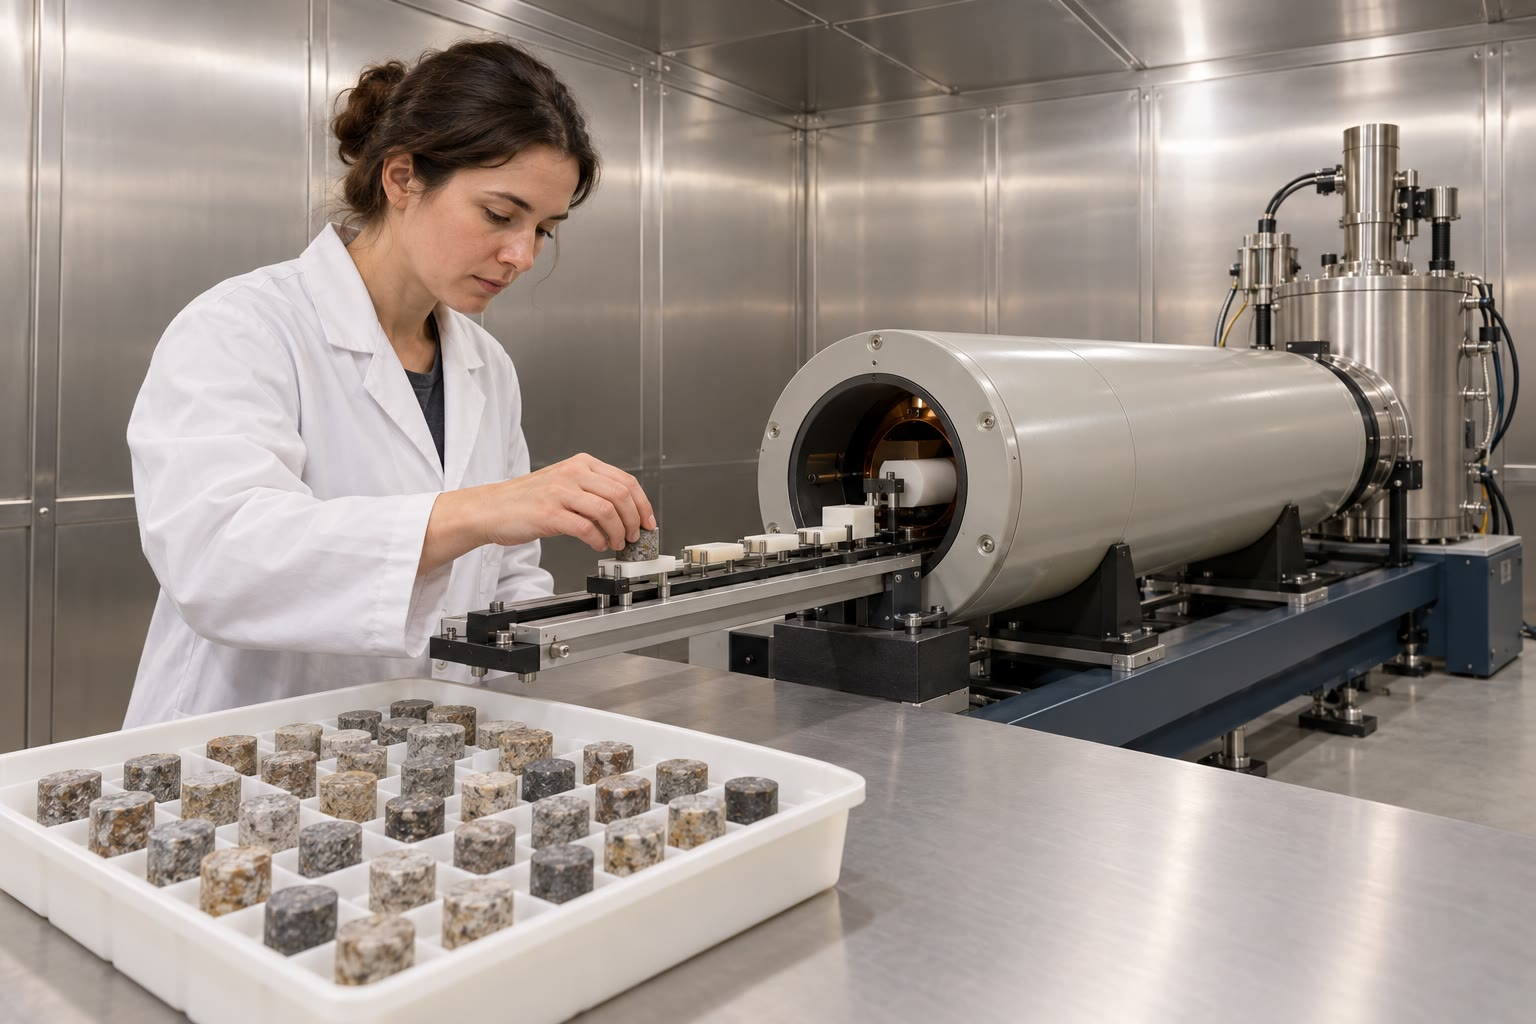
\includegraphics[width=\linewidth]{images/book5/ai/b3-palaeomag-lab.jpg}

{\scriptsize Carregamento de amostras na bandeja de um magnetômetro em uma
sala blindada (ilustração gerada por IA).}
\end{minipage}
\end{inthelab}

\section{Exercícios}

\begin{exercise}[$\star$]\label{exo:b3:palaeomagnetism:1}
Em um campo dipolar axial geocêntrico, calcule a inclinação na latitude
\ang{30}\,N e a latitude de um sítio em que a inclinação é \ang{-20}.
\end{exercise}

\begin{exercise}[$\star$]\label{exo:b3:palaeomagnetism:2}
Em uma estação, o campo tem componentes $X = \qty{20000}{nT}$, $Y =
\qty{-2000}{nT}$ e $Z = \qty{40000}{nT}$. Calcule $H$, $F$, a declinação
magnética e a inclinação.
\end{exercise}

\begin{exercise}[$\star$]\label{exo:b3:palaeomagnetism:3}
Em 2025, $g_1^0 = \qty{-29350}{nT}$. Tomando o campo como um dipolo axial,
calcule o campo no equador e nos polos, e o momento de dipolo
($a = \qty{6371.2}{km}$, $\mu_0 = 4\pi\times\qty{e-7}{H.m^{-1}}$).
\end{exercise}

\begin{exercise}[$\star$]\label{exo:b3:palaeomagnetism:4}
Nomeie o tipo de remanência adquirida e quando ela registra o campo, para: (a) um
derrame de lava que se resfria; (b) silte que se deposita em um lago calmo; (c) um
arenito cujos revestimentos de óxido de ferro se transformam em hematita durante o
soterramento inicial; (d) um basalto que permanece por um milhão de anos no campo atual.
\end{exercise}

\begin{exercise}[$\star\star$]\label{exo:b3:palaeomagnetism:5}
Quatro amostras de um sítio fornecem as direções $(D, I)$: $(\ang{12}, \ang{48})$,
$(\ang{22}, \ang{44})$, $(\ang{16}, \ang{57})$ e $(\ang{6}, \ang{53})$.
Calcule seus vetores unitários, o comprimento da resultante $R$, a direção média, $k$
e $\alpha_{95}$.
\end{exercise}

\begin{exercise}[$\star\star$]\label{exo:b3:palaeomagnetism:6}
Um sítio em \ang{40.0}\,N, \ang{10.0}\,E fornece a direção média $D = \ang{20}$,
$I = \ang{50}$. Calcule sua \omterm{def:b3:palaeomagnetism:vgp}{paleolatitude} e seu \omterm{def:b3:palaeomagnetism:vgp}{polo geomagnético virtual}.
\end{exercise}

\begin{exercise}[$\star\star$]\label{exo:b3:palaeomagnetism:7}
O IGRF fornece um momento de dipolo de \qty{8.32e22}{A.m^2} em 1900 e
\qty{7.69e22}{A.m^2} em 2025, e uma taxa de variação de $g_1^0$ de
\qty{+12.6}{nT/yr} em 2025. (a) Calcule a variação relativa do momento por
século. (b) Se $g_1^0$ mantivesse essa taxa, em quantos anos ele atingiria zero?
Por que isso não é uma previsão?
\end{exercise}

\begin{exercise}[$\star\star$]\label{exo:b3:palaeomagnetism:8}
A remanência restante de uma amostra, em \unit{mA/m} (norte, leste, para baixo), é
$(32.2, 18.1, 38.2)$ após aquecimento a \qty{20}{\celsius}, $(25.8, 18.1, 24.6)$
após \qty{300}{\celsius}, e $(0.0, 0.0, 0.0)$ após \qty{580}{\celsius}; o
\omterm{def:b3:palaeomagnetism:zijderveld}{diagrama de Zijderveld} é retilíneo entre cada par. Calcule a direção e a
intensidade da componente removida entre 20 e \qty{300}{\celsius} e a da
removida acima de \qty{300}{\celsius}. Qual é a ChRM, e qual é a
outra?
\end{exercise}

\begin{exercise}[$\star\star$]\label{exo:b3:palaeomagnetism:9}
Uma formação fornece $I = \ang{-35}$ com $\alpha_{95} = \ang{5}$. Calcule sua
\omterm{def:b3:palaeomagnetism:vgp}{paleolatitude}, a faixa de \omterm{def:b3:palaeomagnetism:vgp}{paleolatitudes} permitida por $I \pm \alpha_{95}$,
e os semieixos $\mathrm dp$ e $\mathrm dm$ da elipse de confiança de seu
polo.
\end{exercise}

\begin{exercise}[$\star\star\star$]\label{exo:b3:palaeomagnetism:10}
(a) A partir do \cref{thm:b3:palaeomagnetism:dipole}, encontre a latitude em que a
inclinação é \ang{45}, e a razão entre o campo nos polos e o campo no equador. (b)
Mostre que $\mathrm dI/\mathrm d\lambda = 2/(1 + 3\sin^2\lambda)$, e deduza onde
um erro de inclinação produz o maior erro de \omterm{def:b3:palaeomagnetism:vgp}{paleolatitude}. (c) Por que as
\omterm{def:b3:palaeomagnetism:vgp}{paleolatitudes} obtidas a partir de inclinações baixas são as mais precisas
em graus?
\end{exercise}

\begin{exercise}[$\star\star\star$]\label{exo:b3:palaeomagnetism:11}
Um local está em \ang{35.0}\,S, \ang{150.0}\,L, em uma placa estável cujo polo de
referência, para a idade de uma formação amostrada ali, está em \ang{70.0}\,N,
\ang{300.0}\,L. (a) Calcule a distância angular $p$ do local ao polo, a
inclinação e a declinação esperadas e a \omterm{def:b3:palaeomagnetism:vgp}{paleolatitude} esperada. (b) A formação
fornece $D_o = \ang{30.0}$, $I_o = \ang{-60.0}$. Calcule a
rotação $R$ e o deslocamento em direção ao polo $P$, e diga o que eles significam.
\end{exercise}

\begin{exercise}[$\star\star\star$]\label{exo:b3:palaeomagnetism:12}
(a) A partir da \cref{prop:b3:palaeomagnetism:fisher}, mostre que a probabilidade de uma direção
estar a menos de $\theta$ da média é $(e^\kappa -
e^{\kappa\cos\theta})/(e^\kappa - e^{-\kappa})$. (b) Para $\kappa$ grande e $\theta$ pequeno,
mostre que isso é aproximadamente $1 - e^{-\kappa\theta^2/2}$, e deduza que
\qty{63}{\percent} das direções estão a menos de $\theta_{63} \approx
\ang{81}/\sqrt\kappa$. (c) Calcule $\theta_{63}$ para $\kappa = 50$, e verifique
os \qty{63}{\percent} com a fórmula exata.
\end{exercise}

\section{Problema: As camadas vermelhas de Kesta}

\begin{problem}[{Problema de fim de semana --- três formações de um terreno deslocado,
suas direções, polos e rotações, e a idade da mais jovem}]
\label{pb:b3:palaeomagnetism:1}
% values: calc/ch04.py; palaeomag_stats.py, magnetostratigraphy.py; GPTS: iodp:gpts2004
Kesta é um terreno fictício, hoje em \ang{47.0}\,N, \ang{15.0}\,L, na borda
de um continente estável fictício. Ele expõe três formações de camadas vermelhas: A,
\qty{60}{Ma}; B, \qty{30}{Ma}; C, de cerca de 3.7 a \qty{2.4}{Ma}. Cada uma foi
amostrada em vários locais, e todo espécime foi desmagnetizado termicamente; a
ChRM é carregada pela hematita, e as formações estão horizontais.

\medskip\noindent\textbf{Parte I --- Direções médias.} Os seis locais da
formação A fornecem $(D, I)$: $(\ang{50}, \ang{37})$, $(\ang{28}, \ang{37})$,
$(\ang{21}, \ang{42})$, $(\ang{24}, \ang{27})$, $(\ang{37}, \ang{39})$,
$(\ang{46}, \ang{38})$.
\begin{enumerate}
  \item Por que uma ChRM carregada por hematita em uma camada vermelha pode ser mais jovem que a
        camada? O que mostraria que ela não é muito mais jovem?
  \item Calcule o vetor unitário da primeira direção.
  \item Os seis vetores unitários somam $(3.8943, 2.6500, 3.5717)$. Calcule $R$ e
        a direção média da formação A.
  \item Calcule $k$ e $\alpha_{95}$ para a formação A.
  \item A formação B fornece, a partir de 7 locais, $D = \ang{23.9}$, $I = \ang{51.5}$ e
        $R = 6.8979$; a formação C, a partir de 8 locais, $D = \ang{3.4}$, $I =
        \ang{63.7}$ e $R = 7.8707$. Calcule $k$ e $\alpha_{95}$ de cada uma.
  \item Qual formação está mais bem agrupada? Qual média está mais bem definida?
\end{enumerate}

\medskip\noindent\textbf{Parte II --- Paleolatitudes e polos.}
\begin{enumerate}[resume]
  \item Calcule as \omterm{def:b3:palaeomagnetism:vgp}{paleolatitudes} de A, B e C.
  \item Para a formação A, calcule a paleocolatitude $p$ e a latitude de
        seu \omterm{def:b3:palaeomagnetism:vgp}{polo geomagnético virtual}.
  \item Calcule a longitude desse polo, verificando qual caso do
        \cref{thm:b3:palaeomagnetism:pole} se aplica.
  \item Calcule $\mathrm dp$ e $\mathrm dm$ para o polo de A.
  \item Os polos de B e C estão em \ang{66.5}\,N, \ang{135.6}\,L e
        \ang{87.1}\,N, \ang{139.1}\,L. Descreva a trajetória dos três polos
        com a idade.
\end{enumerate}

\medskip\noindent\textbf{Parte III --- A idade da formação C.} Na formação C, a partir
da base, os espécimes são reversos até \qty{4.2}{m}, normais até
\qty{14.8}{m}, reversos até \qty{19.7}{m}, normais até \qty{24.6}{m}, reversos até
\qty{29.2}{m} e normais até \qty{54.0}{m}, depois reversos até o topo, em
\qty{64.0}{m}. Um leito de cinza em \qty{22}{m} é datado em cerca de \qty{3.2}{Ma}.
Os subcronos normais do cron C2An abrangem 3.596--3.330, 3.207--3.116 e
3.032--\qty{2.581}{Ma}.
\begin{enumerate}[resume]
  \item Associe as zonas de polaridade com a escala do tempo, usando o leito de cinza.
  \item Calcule a taxa de acumulação entre o primeiro e o terceiro limite de inversão,
        e entre o quarto e o sexto.
  \item Estime as idades da base e do topo da seção.
  \item Por que a taxa é uma média sobre centenas de milhares de anos, e o que
        poderia fazê-la mudar?
\end{enumerate}

\medskip\noindent\textbf{Parte IV --- Contra o continente estável, e a deriva.} Os
polos de referência do continente estável estão em \ang{78.0}\,N, \ang{190.0}\,L
($A_{95} = \ang{3.0}$) a \qty{60}{Ma}; \ang{83.5}\,N, \ang{175.0}\,L
($\ang{2.5}$) a \qty{30}{Ma}; e \ang{87.5}\,N, \ang{150.0}\,L ($\ang{2.0}$)
a \qty{4}{Ma}.
\begin{enumerate}[resume]
  \item Calcule a distância angular de Kesta ao polo de referência de \qty{60}{Ma},
        e a inclinação e a \omterm{def:b3:palaeomagnetism:vgp}{paleolatitude} esperadas.
  \item Calcule a declinação esperada a \qty{60}{Ma}.
  \item As direções esperadas a 30 e \qty{4}{Ma} são $(\ang{2.9},
        \ang{60.0})$ e $(\ang{2.5}, \ang{63.6})$. Calcule o deslocamento
        em direção ao polo $P$ de A, B e C.
  \item Calcule a rotação $R$ de A, B e C.
  \item Calcule os erros $\Delta D_o$ e $\Delta D_x$ para A, e o erro de sua
        rotação.
  \item Os erros de $R$ para B e C são \ang{13.8} e \ang{17.9}. Quais rotações são
        significativas a 95 por cento?
  \item Conte a história de Kesta em relação ao continente estável.
  \item Calcule a deriva para o norte de Kesta desde a formação A, em relação ao
        eixo de rotação, em graus e em quilômetros
        (\qty{111.19}{km} por grau).
  \item Calcule as \omterm{def:b3:palaeomagnetism:vgp}{paleolatitudes} permitidas por $I \pm \alpha_{95}$ para a formação A,
        e tome como um desvio-padrão a metade da largura desse intervalo dividida
        por 1.96. Dê a deriva para o norte de Kesta desde a formação A, em
        quilômetros, com seu desvio-padrão.
\end{enumerate}
\end{problem}
